% !TEX encoding = UTF-8 Unicode

\Chapter{Művészi jellegű szűrők}
A mai világban elég népszerűek az olyan számítógépi vagy mobiltelefonos alkalmazások, amelyek a saját fotóinkat alakítják át. Akár valós időbeli képfeldolgozásról van szó akár videó vagy fotó feldolgozásáról. Ezek nagy része hasonló vagy ugyanazokat az algoritmusokat hasznáják amit én is részletezni fogok a dolgozatomban.
\Section{Népszerű alkalmazási területek}
A fiatalok többsége ha képfeldolgozásról van szó egyből a közösségi média adta lehetőségekre gondolnak ilyen például az Instagram, Snapchat vagy a Messenger alkalmazások. Ezek az applikációk a telefonok, tabletek kamerját használja mint valós idejű mint kép vagy videó feldolgozásra. Ezeknek a programoknak a működését szeretném bemutatni röviden.
\SubSection{Közösségi alkalmazások}
\textbf{Instagram} 
\\
Talán az egyik legismertebb applikáció, ami képekkel és képfeldolgozással foglalkozik azaz Instagram. Ez az alkalmazás pontosan arra készült, hogy a felhasználók megoszthassák egymással a képeiket vagy videóikat amellyeket különböző művészi szűrőkkel láthatnak el. Folyamatosan bővülnek a szűrők, valamit egyre testreszabhatók lesznek a képek/videók, például lehet állítani a képek/videók dőlésszögén, fényességén, hogy mennyire legyen kontrasztos, a színek melegségén, mennyire legyen elmosva és hogy hol legyen elmosva, stb. 
\\
\\ \textbf{Snapchat} 
\\
A Snapchat is egy képfeldolgozással kapcsolatos alkalmazás, bár teljesen más a koncepció mint az Instagramon. Itt is a barátainkkal, imerőseinkkel tudjuk megosztani a képeinket/videóinkat, de ezek a nyilvánosság számára nem láthatók, csak azok láthatják képeinket/videóinkat akiket akarunk, hogy lássák és ők is csak egy bizonyos ideig, amit mi határozunk meg amikor elküldünk egy tartalmat. Ez az alkalmazás nem csak szimplán művészi szűrőkkel foglalkozik, hanem arcdetektálásal. Mivel az alkamazás felismeri az arcunkat, így különböző tárgyakat/ effekteket rak rá az arcunkra, például napszemüveget, vicces sapkákat,  különböző fényeket, eltorzítja az arcunk vagy a szemünket, stb.
\\
\\ \textbf{Messenger} 
\\
Ez az alkalmazás nem kifejezetten képfeldolgozással foglalkozik, azonban már megjelentek benne ezek a funkciók is. Ebben az alkalmazásban barátainkkal, imerőseinkkel tudunk chatelni, képet/videót megosztani, akár privátban, akár csoportosan is. Képeinket/videóinkat hasonló módon tudjuk szerkeszteni mint a Snapchat alkalmazással. Itt is arcfelismerés alapján tud rárakni az arcunkra a program mindenféle effektet, például szemüvegeket, sapkákat, fényeket, stb. Ebben programban elérhető a videóhívás is ahol szintén haszálhatóak ezek az effektek.
\begin{figure}[ht]
\centering
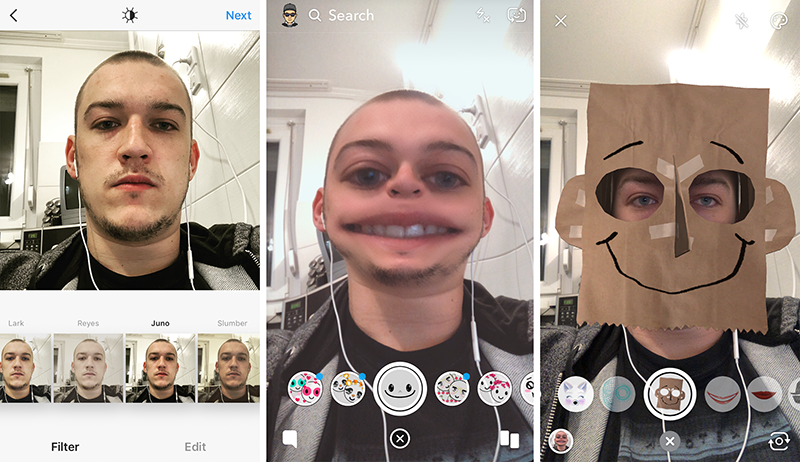
\epsfig{file=kepek/instasnapmess.png,scale=0.47}
\caption{Instagram, Snapchat, Messenger képernyőfotók } 
\label{fig: instagram, snapchat, messenger}
\end{figure}
\SubSection{Webcamera-, mobil alkalmazások}
A közösségi alkamazásokon kívül, van néhány olyan weboldal, mobil alkalmazás ami képfeldolgozással foglalkozik. Ezek az alkalmazások általában csak képekre tudnak művészi szűrőket rátenni. Az első amit szeretnék megemlíteni az egy mobil alkalmazás aminek a neve Prisma. 
\\
\\ \textbf{Prisma}
\\
Ez az alkalmazás a képfeldolgozáshoz mesterséges intelligenciát valamit a neurális hálókat haszánálja, hogy művészi fiterekkel ellátott képeket hozzon létre, normál fotókból. A felhasználó az alkalmazásba betölti az átalakítandó fényképet, kiválasztja a számára megfelelő szűrőt, pár másodperc mulva a szűrővel elláttott kép megjelenik az alkalmazásban. A képfeldolgozás a Prisma szerverein történik, ott történik a mesterséges intelligencia továbbá a neurális hálók használata. %wikipedia
\\
\\ \textbf{Webcamera alkalmazások} 
\\
Számtalan olyan program, weblap van ami képfeldolgozással foglalkozik. Léteznek gyári beépített programok, ami a webcamera saját illesztőprogramjában található meg, és különböző szűrőket tud rárakni a képekre. Weboldalak is foglalkoznak ezzel a területtel, több olyan webalkalmazást találtam, ami hasonló megoldásokat használ képátalakításra mint amit én fogok a továbbiakban.
\begin{figure}[ht]
\centering
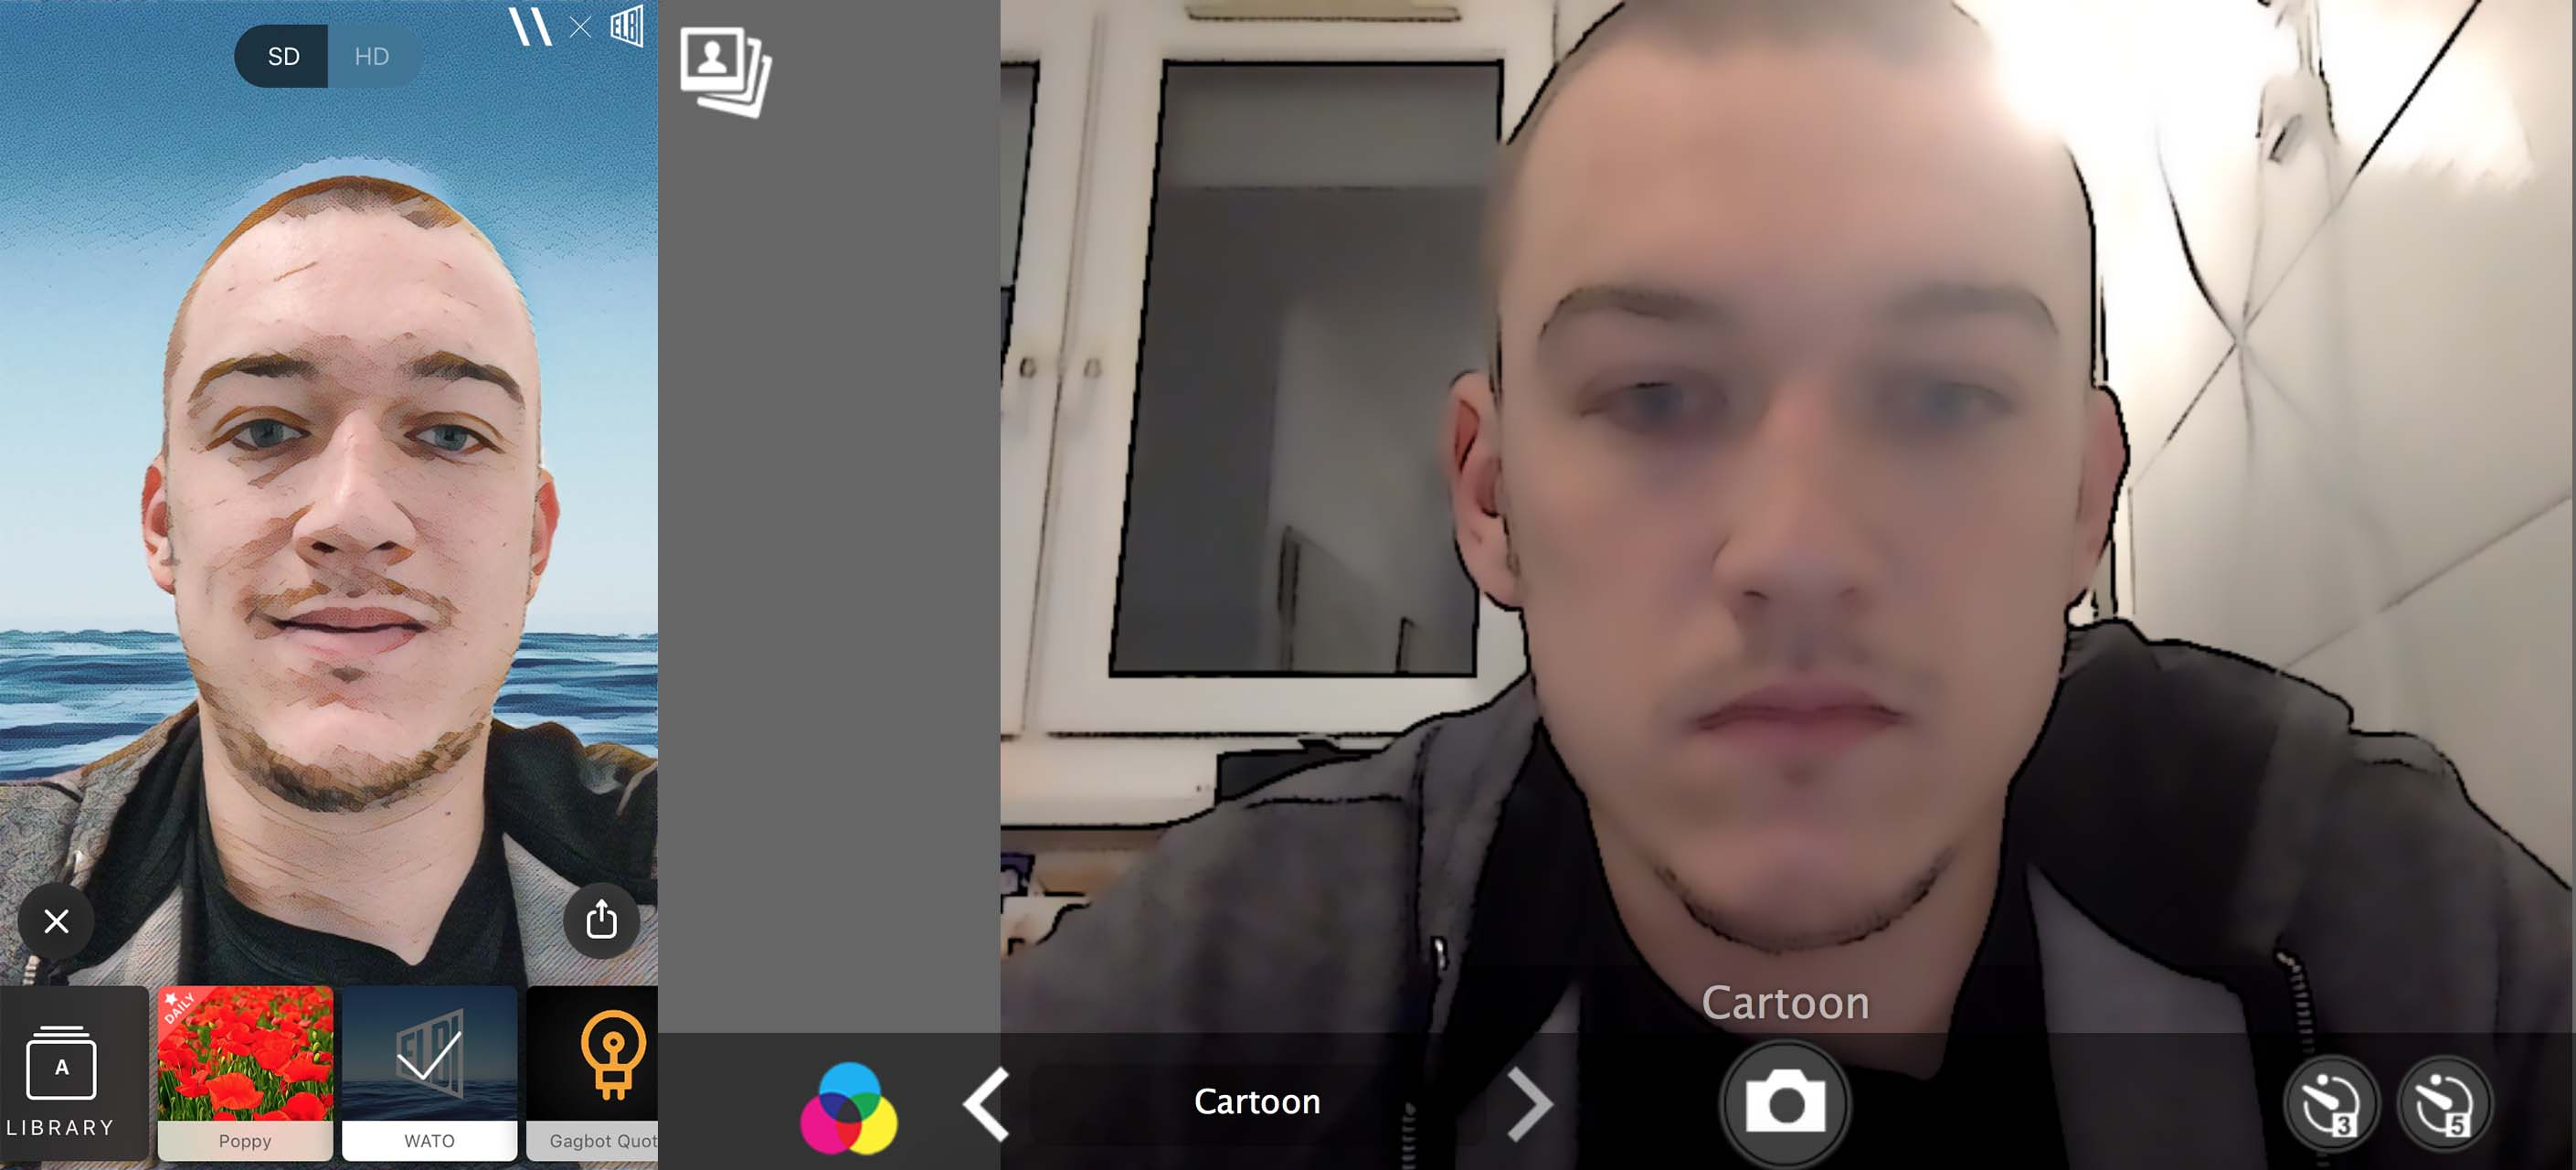
\epsfig{file=kepek/prismawebcam.jpg,scale=0.3}
\caption{Prisma,  https://www.pixect.com képernyőfotók} 
\label{fig: JetSetRadio}
\end{figure}
% https://www.pixect.com képernyőfotók
\SubSection{Filmek, játékok amelyekhez művészi szűrőket használtak}
Művészi jellegű szűrőket nem csak magán felhasználók használnak arra, hogy boldogítsák magukat valamint barátaikat a jobbnál jobb képekel, videókkal, hanem ilyen filtereket használtak például videójátékok emellett filmek készítésére is.
\\
\\
\\ \textbf{Jet Set Radio videójáték} 
\\
Ez volt a világon az első olyan videójáték amelyen sötét árnyalatú grafikákat mutattak be, túlzott alakokkal, vastag vonalakkal és lapos, élénk színekkel. Ezzel olyan érzetet keltve mintha egy képregény vagy egy mese lenne. A játékban egy görkorcsolyást kell irányítani és graffitiznie kell a megadott helyekre mielőtt lejár az idő, plusz pontokért lehet mindenféle extrém trükköt is csinálni korizás közben. Nehezítésként a játékost üldözik gyalogosan, helikopterekkel és tankokkal.%wikipedia
\\
\\
\textbf{Kamera által homályosan (A Scanner Darkly) c. film} 
\\
A filmet digitálisan forgatták, majd interpolált rotoszkóp segítségével animálták. Ez egy olyan animációs technika, melyben az eredeti felvételekből képkockáról képkockára filtereztek. Ezzel olyan hatást értek el, hogy azt lehet mondani erre a filmre, hogy animációs film. A film röviden, nem is olyan távoli jövőben az Egyesült Államok lakosságának nagy része kábítószer-fogyasztó. A hatalom beépített titkos ügynökök és hatékony megfigyelési rendszerek segítségével próbálja az ellenőrzést fönntartani. Az egyik nyomozót, Fredet megbízzák, hogy álljon rá Bob Arctor dílerre, aki életveszélyes drogot terjeszt. Ennek mellékhatásaként ugyanis az ember személyisége két, egymással ellentétes félre bomlik. Fred rájön, hogy Arctor valójában az ő alteregója és önmaga megfigyelése a technikai kérdéseken túl komoly pszichológiai kihívásokat is felvet. % wikipedia, Port.hu
\begin{figure}[ht]
\centering
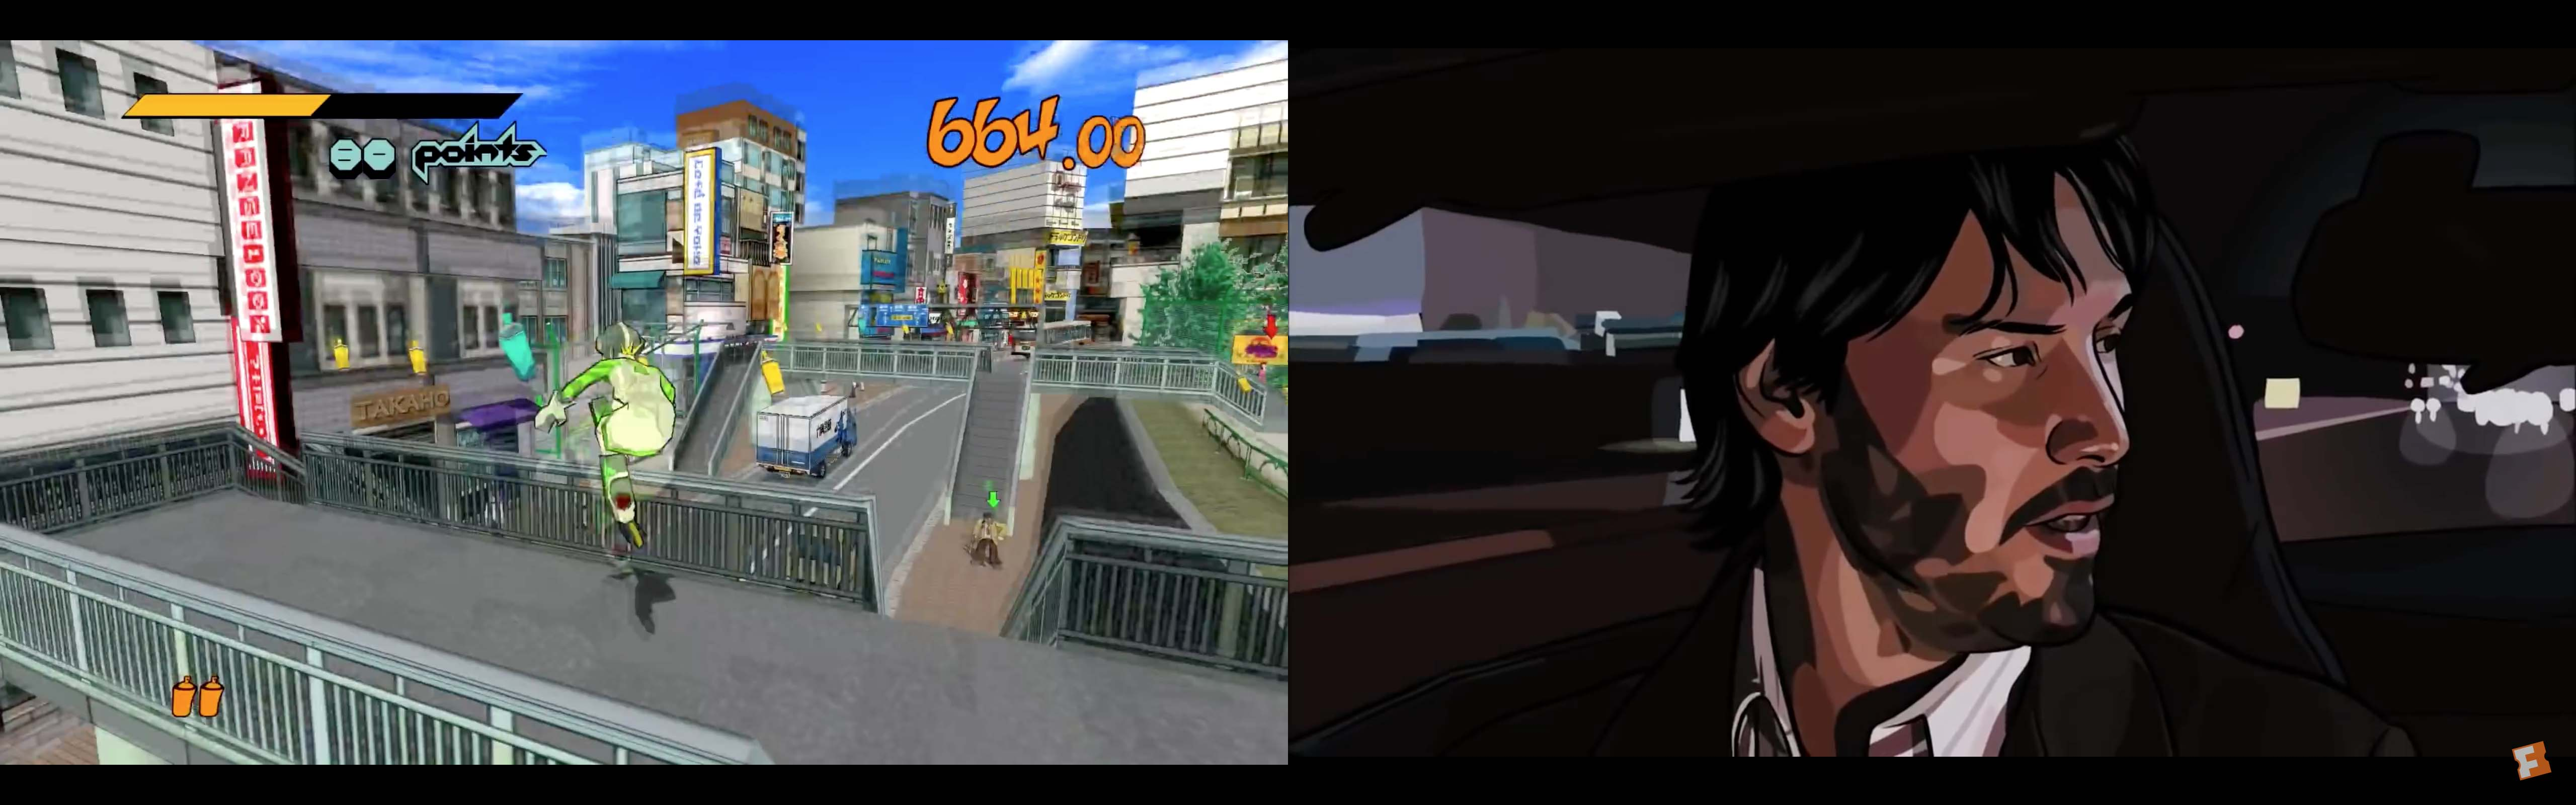
\epsfig{file=kepek/jatekfilm,scale=0.17}
\caption{Jet Set Radio videójáték és Kamera által homályosan c. film képernyőfotó} 
\label{fig: Jatek, film}
\end{figure}
%Közösségi alkalmazások (Snapchat, Instagram, ...)
%Hardverbe integrált, webkamera alkalmazások
%Filmek
%Játékok
\Section{Megvalósítás nehézségei}
A digitális képfeldolgozás számítógépes algoritmusokat használ a digitális képek készítéséhez. Ez lehetővé teszi, hogy sokkal szélesebb körű algoritmusokat alkalmazzanak a bemeneti adatokra, és ezekkel az algoritmusokkal elkerülhetők az olyan problémák, mint a zaj és a jelek torzulása a feldolgozás során. Mivel a képeket két dimenzióban definiálják (talán több dimenzióban is), a digitális képfeldolgozást multidimenzionális rendszerek formájában lehet modellezni.  Ezekkel a képfeldolgozási algoritmusokkal lehet olyan képeket készíteni, amiket például azok az alkamazások is létrehoznak amiket ebben a fejezetben bemutattam.
%Konvolúciós módszer 
%https://en.wikipedia.org/wiki/Digital_image_processing
\Section{Elvárások a szűrőkkel kapcsolatban}
Olyan szűrőket szeretnék létrehozni, amelyek hasonlóképpen működnek, mint azok az applikációk, játékok, filmek amiket ebben a fejezetben említem. Cartoon jellegű, festmény szerű valamint ceruza rajz jellegű szűrőket szándékozok létrehozni, amiket  képeken, videókon ezekután valósidőben is tesztelni fogok. 


 %3-4 oldal